%%%%%%%%%%%%%%%%%%%%%%%%%%%%%%%%%%%%%%%%%%%%%%%%%%%%%%%%%%%%%%%%%%%%%%%%%%%%%%%%
%2345678901234567890123456789012345678901234567890123456789012345678901234567890
%        1         2         3         4         5         6         7         8

\documentclass[letterpaper, 10 pt, journal, twoside]{IEEEtran}  % Comment this line out if you need a4paper

%\documentclass[a4paper, 10pt, conference]{ieeeconf}      % Use this line for a4 paper

\IEEEoverridecommandlockouts                              % This command is only needed if 
                                                          % you want to use the \thanks command

%\overrideIEEEmargins                                      % Needed to meet printer requirements.

% The following packages can be found on http:\\www.ctan.org
\usepackage{graphics} % for pdf, bitmapped graphics files
\usepackage{graphicx}
\usepackage{amsmath,amssymb,latexsym,float,epsfig,subfigure}
\usepackage{amsmath} % assumes amsmath package installed
\usepackage{amssymb}  % assumes amsmath package installed
\usepackage{lipsum}
\usepackage[export]{adjustbox}
\usepackage[normalem]{ulem} % underline
\usepackage{wrapfig}
\usepackage{multirow}
\usepackage{balance}
\usepackage{color}
\usepackage{url}

\title{
	Human-in-the-Loop Optimization of Shared Autonomy in Assistive Robotics
}

\author{Deepak Gopinath$^{1,3}$, Siddarth Jain$^{2,3}$, and Brenna D. Argall$^{1\text{-}4}$%
	\thanks{Manuscript received: March, 1, 2016; Revised June,
		7, 2016; Accepted June, 29, 2016.}%Use only for final RALversion
	\thanks{This paper was recommended for publication by Editor
		Ken Masamune upon evaluation of the Associate Editor and
		Reviewers' comments. Research reported in this publication was supported by the
		NIBIB \& NICHD
		under award number R01EB019335.}%Use only for final RAL version
	\thanks{$^{1}$Deepak Gopinath and Brenna D. Argall are with Department of Mechanical Engineering, Northwestern University, Evanston, IL, 60208, USA
		{\tt\small deepakedakkattilgopinath2015@u.northwestern.edu}}%
	\thanks{$^{2} $Siddarth Jain and Brenna D. Argall are with Department of Electrical Engineering, Northwestern University, Evanston, IL, 60208, USA {\tt\small sidd@u.northwestern.edu, brenna.argall@northwestern.edu }}%
	\thanks{$^{3} $Deepak Gopinath, Siddarth Jain and Brenna D. Argall are with Rehabilitation Institute of Chicago, Chicago IL, 60211 USA}%
	\thanks{$^{4} $Brenna D. Argall is with Department of Physical Medicine and Rehabilitation, Northwestern University, Chicago, IL, 60611 USA}%

	\thanks{Digital Object Identifier (DOI): see top of this page.}
}
\begin{document}
	\maketitle
	\markboth{IEEE Robotics and Automation Letters. Preprint
		Version. July, 2016}
	{Gopinath \MakeLowercase{\textit{et al.}}:
		Human-in-the-loop}
%	\thispagestyle{empty}
%	\pagestyle{empty}
	
	
	%%%%%%%%%%%%%%%%%%%%%%%%%%%%%%%%%%%%%%%%%%%%%%%%%%%%%%%%%%%%%%%%%%%%%%%%%%%%%%%%
		\begin{abstract}
			In this paper, we propose a mathematical framework which formalizes user-driven customization of shared autonomy in assistive robotics as a nonlinear optimization problem. 
			Our insight is to allow the \textit{end-user}, rather than relying on standard optimization techniques, to perform the optimization procedure, thereby allowing us to leave the exact nature of the cost function indeterminate.
			We ground our formalism with an interactive
			optimization procedure that customizes
			control sharing using an assistive robotic arm. We also present
			a pilot study that explores interactive optimization with
			end-users.
			This study was performed with 17 subjects (4 with spinal cord injury, 13 without injury). Results
			show all subjects were able to converge to an assistance paradigm, suggesting the existence of optimal solutions. Notably, the amount of assistance was not always
			optimized for task performance. Instead, some subjects
			favored retaining more control during the execution over better task
			performance.
			The study supports the case for user-driven customization and provides
			guidance for its continued development and study.
		\end{abstract}
	\begin{IEEEkeywords}
	Rehabilitation Robotics; Physically Assistive Devices; Human Factors and Human-in-the-Loop
	\end{IEEEkeywords}
		
	%%%%%%%%%%%%%%%%%%%%%%%%%%%%%%%%%%%%%%%%%%%%%%%%%%%%%%%%%%%%%%%%%%%%%%%%%%%%%%%%
	\section{INTRODUCTION} \label{Intro}
	
	\IEEEPARstart{F}{or} people with severe motor impairments as a result of spinal cord or
	brain injuries, assistive and rehabilitation machines such as
	assistive robotic arms, upper or lower limb prostheses and powered
	wheelchairs are crucial for reducing their dependence on caretakers
	and increasing the ability to perform activities of daily life. 
	However, for many, the control of such devices remains a
	challenge---for example, due to their physical impairments or limitations of the control interfaces. Limited interfaces issue control signals that are low-dimensional, discrete and operate in modes which correspond to different parts of the control space that must be switched between. The introduction of
	partial autonomy to these devices---in which the control is shared
	between the human and robotics autonomy---aims to help reduce the cognitive and physical burden on the user. 
	
	The reduced bandwidth of the control signals generated by motor-impaired users makes them more reliant on the interaction with the autonomy, and also less adaptable and more vulnerable to any arbitrariness present in the system---for example, the choice of control interfaces and mappings, or the exact specification of how control is shared between the user and the autonomy. A thorough analysis of user performance and the differences in performance between uninjured and motor-impaired subjects calls for a rich mathematical framework that can capture the various facets of the shared control system, like the complex dynamics of the human-robot interaction. \textit{Furthermore}, the exact formulation used to describe the human-robot interaction will determine (or limit) the relevant and valid questions that can be 
	asked and how the analysis of performance metrics will be performed. To accomplish this, we introduce a mathematical formalism in which the customization procedure is formulated as a nonlinear optimization problem over system parameters. 
	
	Since users differ in their
	physical abilities and desired amount of assistance, \textit{customization} of the amount of assistance is critical for the adoption of assistive shared-control systems.
	Predefined assistance levels 
	can provide good starting points but may not remain optimal for the user in the long term. For example, the subject's abilities will likely be changing---either degrading (e.g.~due to degenerative disease) or improving (e.g.~due to successful rehabilitation). As a result, the need for assistance may increase or decrease. One way to accomplish customization is to tune the system parameters which will bring about a change in the human-robot interaction and the final behavior. The aim is to optimize the human-robot interaction during task performance. A straightforward choice of optimality criterion is to consider task-related performance metrics such as minimizing the time taken and energy expended. Such metrics however may not capture user-related metrics like comfort, independence or satisfaction.
	
	Our insight is that if we entrust the task of customization to the users, they likely will tune the system in such a way that the optimal interaction---according to their personal optimality criterion---will emerge. Moreover, the user-driven customization of assistance may be user-dependent in addition to being task-dependent. 
	
	To ground our formalism, we present a first implementation, in which the reasoning between the user control
	and the robot policy is a function of confidence in the inference of human intent, with tunable parameters. 
	Our interactive user-driven customization system maps verbal cues from the human to adjustments
	in these parameter values. Results from an exploratory pilot study also are presented.
	
	In Section~\ref{rw} we present an overview of the relevant research in
	the field of shared control systems in assistive
	technology. Section~\ref{pf} overviews of the general algorithm and
	system design used in this study. The system implementation is
	described in Section~\ref{si} and Section~\ref{PSM} provides
	an overview of the
	user study methods, tasks and metrics used. 
	In Section~\ref{RES} we present the results from our pilot study and discussion followed by conclusions in Section~\ref{CON}.
	
	\section{RELATED WORK} \label{rw}
	
	
	The introduction of robotics autonomy to assistive devices
	can offload some control burden from users to enable
	easier operation. While full autonomy is an option, more common are systems that share control with the human user---for reasons of both robustness~\cite{05icorr-volosyak} and user preference~\cite{01smc-kim}.
	
	The most common methods to share control
	between the user and autonomous system include (a) the user
	selects the higher-level goal and the autonomy generates
	the lower-level control, (b) control partitioning schemes and (c)
	blending the user controls and the autonomy commands.
	In the domain of robotic wheelchair research, the higher-level goals typically are navigation goals~\cite{05jrrd-simpson}, while control
	partitioning for example places the control of speed with the user
	and heading with the autonomy~\cite{NAVCHAIR}. Control
	blending paradigms often are employed for behaviors like
	obstacle avoidance~\cite{12smc-carlson}. Control sharing in case of robotic arms
	most commonly involves user-specification of a target (such
	as an object)~\cite{jain2010assistive} or pose correction~\cite{04ar-bien}, and the robot autonomously generates the motion commands. 
	Approaches that partition the control space
	may, for example, place the control of end-effector position in
	$z$ with the human and in $x,y$ with the autonomy~\cite{05uais-driessen}.
	Control blending is less straightforward---because the user rarely is able to issue a control signal with high enough dimensionality to cover all control dimensions of the robot (e.g. 6D)---but recently is gaining interest.
	
	Moreover, there are approaches which study specifically the customization of how this control blending happens~\cite{ li2011dynamic}. The amount of control blending often is determined using an arbitration function that is based, for example, on the autonomy's confidence in its prediction of the user's goal~\cite{dragan2012formalizing}. Our work similarly employs an arbitration function to dictate the amount of control sharing. 
	
	
	Optimization techniques have been adopted to generate different strategies for control sharing; for example, formulating the problem as a POMDP and inferring a distribution over goals~\cite{javdani2015shared}, using pseudo-navigation functions for collaborative control~\cite{fernandez2015towards} or concatenating energy-optimal motion primitives to create optimal trajectories~\cite{lawitzky2013trajectory}. Although these approaches result in improved task performance (completion time, control effort), the assistance schemes are mixed in terms of user acceptance. In particular, there are instances of assistance resulting in higher user dissatisfaction~\cite{javdani2015shared}, and users preferring to be in control and more cautious~\cite{lawitzky2013trajectory}. In other studies users find the assistance at times to be uncooperative and tolerate a loss of control only for a significant improvement in performance~\cite{you2012assisted}.
	
	In an attempt to construct more realistic cost functions, others inspired by design research incorporate a measure of ``discomfort" into the optimization cost function~\cite{gulati2009framework}. However, the specific form of the cost function is domain dependent and is not generalizable to other assistive devices such as robotic arms. 
	
	Despite an improvement in task performance, none of the above cost function formulations were able to guarantee high user satisfaction (with the exception of domain-specific discomfort~\cite{gulati2009framework}). The need for higher user satisfaction is crucial for the acceptance of robot autonomy by the end-users in the assistive domain. This gap motivates our approach to engage the end-user in the optimization procedure.
	
	\section{PROPOSED FRAMEWORK} \label{pf}
	
	Principles from optimal control theory have been successfully used to account for different aspects of human motor control such as  arm trajectory formation, posture control and locomotion \cite{ uno1989formation, flash1985coordination,todorov2004optimality}.
	The underlying motivation in using optimal control theory is that biological systems have evolved to produce motor commands which will optimize motor behavior with respect to the task at hand \cite{todorov2004optimality}. When a human operates an assistive robot to replace his/her lost motor function, the extension of this reasoning is that the optimizing principles are operating over control commands to the robot effector rather than motor commands to the human muscles.
	We frame our formalism within the language of optimal control theory not only because of this biological parallel, but also because it will allow for the analysis of the effects of the various design decisions in and components of a shared control system in a thorough and rigorous manner. 
	
	\subsection{Formalism}
	Let $\boldsymbol{x}(t)$ denote the state of the system at time $t$. 
	Let $\boldsymbol{\theta}(t)$ be the set of tunable parameters that will affect the amount of control shared between the human and the robot. 
	The other control inputs to the system are $\boldsymbol{u}_h(t)$ and $\boldsymbol{u}_r(t)$, the control commands generated respectively by the user and autonomous robot policy at time $t$. 
	
	The control signal from the robot autonomy is generated by a function $f_{r}(\cdot) \in \mathcal{F}_{r}$, 
	\begin{equation}
	\boldsymbol{u}_r(t) \leftarrow f_{r}(\boldsymbol{x}(t))
	\end{equation}
	where $\mathcal{F}_{r}$ is the set of all control behaviors corresponding to different tasks.
	
	We assume that the control command $\boldsymbol{u}_h(t)$ is generated by a function of  $f_{h}(\cdot) \in \mathcal{F}_{h}$,
	\begin{equation}
	\boldsymbol{u}_h(t) \leftarrow f_{h}(\boldsymbol{x}(t))
	\end{equation}
	where $\mathcal{F}_{h}$ is the set of user behaviors corresponding to different tasks. $f_{h}(\cdot)$ is simply a symbolic representation of the mapping function that generates $\boldsymbol{u}_{h}(t)$ and is completely unknown to the autonomous system.
	The sole dependence of $\boldsymbol{u}_h(t)$ on $\boldsymbol{x}(t)$ is an approximation because there may be a large number of unobserved variables (e.g.~fatigue or personal satisfaction) affecting the user's control. 
	
	The shared control system makes use of function $\boldsymbol{\beta}(\cdot)$, parameterized by $\boldsymbol{\theta}$
	\begin{equation}
	\boldsymbol{u}(t) \leftarrow \boldsymbol{\beta}_{\theta}(\boldsymbol{u}_h(t), \boldsymbol{u}_r(t))
	\end{equation}
	which arbitrates between the control commands from the user and the robot policy to produce control command $\boldsymbol{u}(t)$ executed by the robot.
	
	A key insight in our formulation is that, for a time--varying function $\boldsymbol{\beta}(\cdot)$, the parameters themselves can be functions of time and therefore may be interpreted as control signals. Then the dynamics of the system can be written as
	\begin{equation}
	\boldsymbol{\dot{x}}(t) \leftarrow \boldsymbol{a}(\boldsymbol{x}(t), \boldsymbol{\theta}(t), \boldsymbol{u}_h(t), \boldsymbol{u}_r(t), t)
	\end{equation}
	where $\boldsymbol{a}(\cdot)$ is in general a nonlinear, time-varying function. Note that in this formulation the parameters $\boldsymbol{\theta}(t)$ are treated in the \textit{same way} as the other control signals.
	The problem of finding the set of parameters $\boldsymbol{\theta}(t)$ that will generate the optimal human-robot interaction and task performance (as determined by a cost function) thus may be formulated as an optimal control problem.
	
	Optimal control models assume the existence of some kind of cost function being optimized during task performance.\footnote{For example, arm trajectories generated by uninjured humans during reaching tasks are reproduced using cost functions composed of torque generated at the joints~\cite{uno1989formation} or jerk of the end effector (hand)~\cite{flash1985coordination}.} In general, the cost function $\boldsymbol{J}$ can be written as,  
	\begin{equation}
	\boldsymbol{J} \leftarrow \boldsymbol{h}(\boldsymbol{x}(t_f), t_f) + \int\limits_{t_0}^{t_f} \boldsymbol{k}(\boldsymbol{x}(t), \boldsymbol{u}(t), t)dt
	\end{equation}
	where the first term corresponds to a terminal cost (e.g~proximity of the end pose to the target pose) and the second term corresponds to a measure of internal cost (e.g~energy expended, completion time, etc). The true cost function however likely is more complex, and could include additional factors such as user satisfaction. The state boundary conditions are given by 
	$
	\boldsymbol{x}(t_0)	= x_0 
	$ and
	$
	\boldsymbol{x}(t_f) = x_f
	$,
	where $t_0$ and $t_f$ are the times at which the robot is in the initial state $x_0$ and final state $x_f$. 
	The parameter constraints are
	$
	\boldsymbol{\theta}_{min} \leq \boldsymbol{\theta}(t) \leq \boldsymbol{\theta}_{max}
	$.
	
	The elements of the framework $f_{r}(\cdot)$, $f_{h}(\cdot)$, $\beta(\cdot)$ and 
	$a(\cdot)$ are system-specific, and different choices of these functions will have drastically different impact on task performance and user satisfaction. Moreover, the impact is anticipated to be all the greater on motor-impaired subjects.
	\begin{figure}
		\begin{center}
			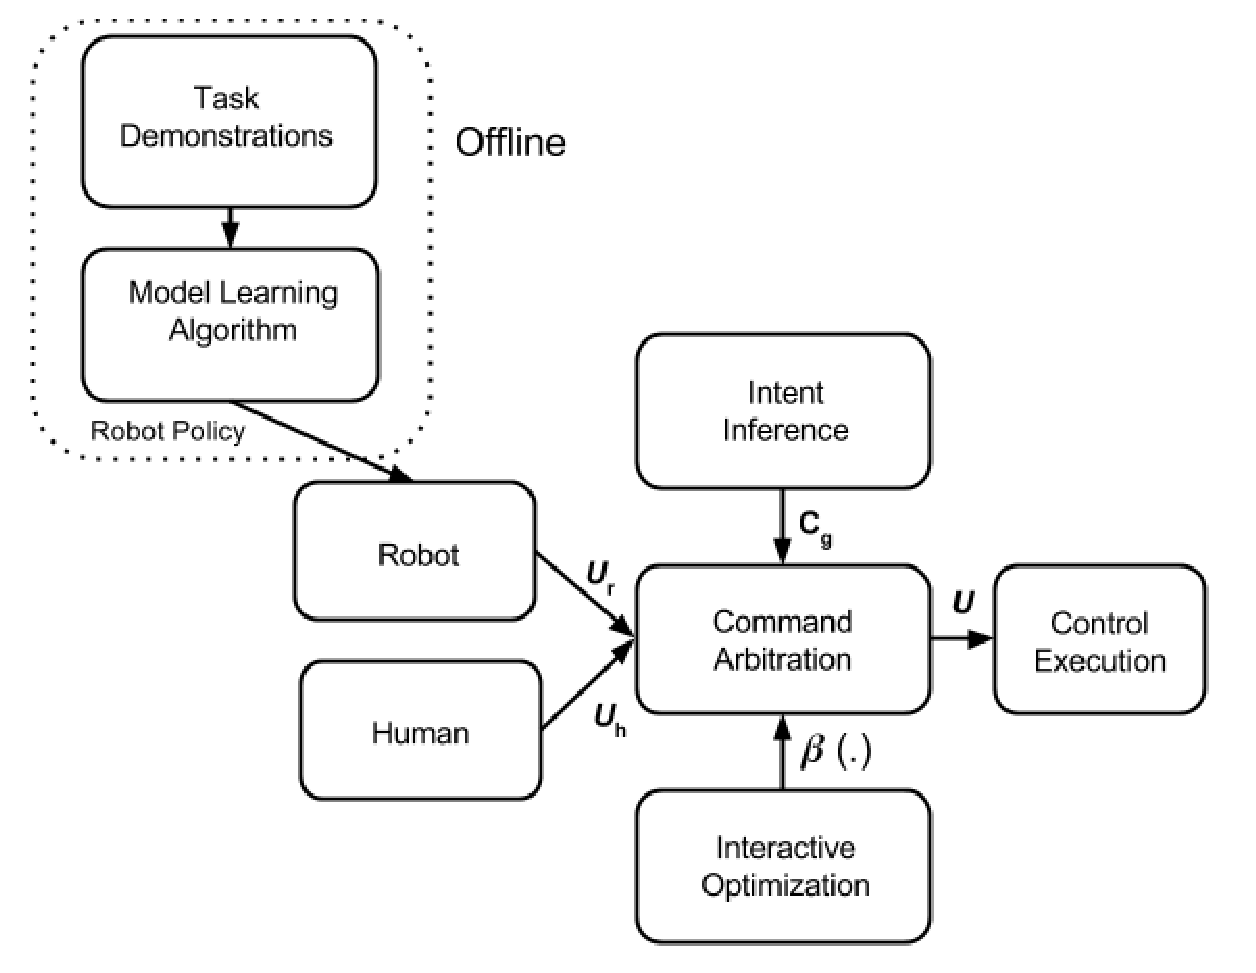
\includegraphics[width = 1\hsize]{./finalfigures/Figure1.eps}
			\vspace{-0.5cm}
			\caption{System design. Core components include command arbitration
				and the interactive optimization of how this arbitration happens.}
			\label{SD}
		\end{center}
	\end{figure}
	\subsection{Optimization}
	Typically optimization is performed over all control signals that are inputs to the system. In our system, however, the control commands from the human and the robot ($ \boldsymbol{u}_h(t), \boldsymbol{u}_r(t)$) are treated as given quantities, and the goal rather is to optimize the interaction parameters $\boldsymbol{\theta}(t)$. 
	
	In this work, we furthermore make no attempt to determine the exact nature of the cost function $\boldsymbol{J}$. There might be a myriad of unmeasurable factors influencing the cost function, and determining the exact mathematical form for the cost function likely is an intractable problem. Making any kind of approximation to simplify the cost function in turn will affect the robustness and efficacy of the assistive system. Since we do not want to reduce the assistive capabilities of our system, and we have a human in the loop, our insight is that the optimization task can be performed by the user him/herself, instead of adopting standard nonlinear optimization algorithms. Thus there is no need to concretely define $J$ and the user tunes the parameters $\boldsymbol{\theta}(t)$ until the desired behavior is achieved. 
	
	In this user-driven customization system, the overall effect of parameter tuning is that of changing the assistance offered by the robot. The specific optimization procedure is described in detail in Section \ref{UDOAP}.	
	
	\section{SYSTEM IMPLEMENTATION} \label{si}
	
	
	Our system implementation is overviewed in Figure~\ref{SD}. 
	The key components of this system include the command arbitration paradigm (Sec. \ref{CA}),
	the user-driven optimization procedure (Sec. \ref{UDOAP}) and the estimation of human intent (Sec. \ref{ECV}).
	Also provided are details of how the human control signals are acquired (Sec. \ref{CIM}) and the robot autonomy
	commands are generated (Sec. \ref{DRP}). 
	
	\subsection{Command Arbitration} \label{CA}
	
	In our implementation, the function $\beta(\cdot)$ that reasons between the robot and human control signals
	is a linear blending function,
	\begin{equation}
	\beta_{\boldsymbol{\theta}}(\boldsymbol{u}_{\textit{h}}(t),\boldsymbol{u}_{\textit{r}}(t)) \triangleq (1-\alpha_{\boldsymbol{\theta}}) \cdot \boldsymbol{u}_{\textit{h}}(t) +  \alpha_{\boldsymbol{\theta}} \cdot \boldsymbol{u}_{\textit{r}}(t) %\newline
	\label{eq:blend}
	\end{equation}
	where $\alpha_{\boldsymbol{\theta}} \in [0,1]$ is itself a function parameterized by $\boldsymbol{\theta}$.\footnote{The time index $t$ is dropped from $\boldsymbol{\theta}(t)$ for brevity in notation.}
	Note that $\alpha_{\boldsymbol{\theta}}=0$ corresponds to full teleoperation,
	and $\alpha_{\boldsymbol{\theta}}=1$ to full autonomy.
	
	The majority of \textit{arbitration functions} $\alpha_{\boldsymbol{\theta}}$ can be reduced to the functional
	form pictured in Figure~\ref{PAF} \cite{dragan2012formalizing}, characterized by a set of three parameters $\{\theta_{1}, \theta_{2}, \theta_{3}\}$ and independent variable $c(t)$. The parameter set determines:
	\begin{itemize}
		\item $\theta_{1}$: The minimum value of $c(t)$ above which control blending is performed. 
		\vspace{0.1cm}
		\item $\theta_{2}$: The value of $c(t)$ above which the blending parameter is maximum and constant. 
		\vspace{0.1cm}
		\item $\theta_{3}$: The maximum value of $\alpha$ for any value of $c(t)$. 
		\vspace{0.1cm}
	\end{itemize}
	
	\begin{wrapfigure}[12]{R}{0.27\textwidth}
		\begin{center}
			\vspace{-.6cm}
			\includegraphics[width=0.27\textwidth]{./finalfigures/Figure2.eps}
		\end{center}
		\vspace{-.45cm}
		\caption{A prototypical arbitration function, parameterized by {\footnotesize $\boldsymbol{\theta} = \{\theta_{1}, \theta_{2}, \theta_{3}\}$}.}
		\label{PAF}
	\end{wrapfigure}
	Note that $\theta_{3}$\;=\;$0$ corresponds to constant teleoperation (irrespective of the value of $c(t)$). The relationship between $c(t)$ and $\alpha_{\boldsymbol{\theta}}$ is linear between $\theta_{1}$ and $\theta_{2}$, and the slope of this linear relation determines how aggressively the robot assumes control.
	The parameter bounds are such that $\forall i,~ \theta_{i}(t) \in [0,1]$ and $\theta_{1} \leq \theta_{2}$.
	The independent variable $c(t)$ in our implementation is discussed in Sec \ref{ECV}. 
	
	In our pilot study, the parameters were tuned only between tasks and were unchanged during task execution, and so $\boldsymbol{\theta}_{i}(t) = \boldsymbol{\theta}_{i}(t_{0}),\; \forall t \in [t_{0}, t_{f}]$.
	The arbitrated signal $\boldsymbol{u}(t)$ was the velocity of the end-effector in Cartesian space, converted to joint-space velocities via inverse kinematics.
	\subsection{User--Driven Optimization of the Arbitration Parameters} \label{UDOAP}
	
	In this first exploration of our interactive optimization
	procedure, verbal commands from the human subject are translated to changes in $\boldsymbol{\theta}$ by the system operator. The interactive optimization procedure is currently being formalized and automated, as informed by this pilot data. 
	
	A change in assistance level can be achieved by modulating one or more of the $\theta_{i} \in \boldsymbol{\theta}$, according to
	$\theta_{i} = \theta_{i} \pm \delta\theta_{i}$.
	In our implementation, at initialization $\delta\theta_{i} =
	0.1$.
	The value of $\delta\theta_{i}$ is adaptive, and is halved if a request to increase assistance is immediately followed by a request to decrease and vice versa (in order to avoid oscillatory behavior). 
	
	\begin{table}[t]
		\centering
		\begin{tabular}{|l|l|l|}
			\hline
			{Verbal Cue} & {Parameters Changed} & {Amount of change}\\
			\hline
			``More'' & $\theta_{3}\uparrow$, $\theta_{2}\downarrow$, $\theta_{1}\downarrow$ & $\delta\theta \leftarrow \delta\theta$
			\\ \hline
			``Less'' & $\theta_{3}\downarrow$, $\theta_{2}\uparrow$, $\theta_{1}\downarrow$ &  $\delta\theta \leftarrow \delta\theta$ \\ \hline
			``Little More'' & $\theta_{3}\uparrow$, $\theta_{2}\downarrow$, $\theta_{1}\uparrow$ & $\delta\theta \leftarrow \frac{1}{2} \delta\theta$ \\ [5pt] 	 \hline
			``Little Less'' & $\theta_{3}\downarrow$, $\theta_{2}\uparrow$, $\theta_{1}\;(no\;change)$  & $\delta\theta \leftarrow \frac{1}{2} \delta\theta$ \\  \hline
		\end{tabular}
		\label{tbl:maptable}
		\vspace{.2cm}
		\caption{Mappings from verbal cues to parameters changed}
		\vspace{-.4cm}
		($\uparrow$ indicates a positive $\delta\theta$ and $\downarrow$ denotes a negative $\delta\theta$)
		\vspace{-0.2cm}
	\end{table}
	Table I provides a few example mappings between common
	verbal cues, the parameters changed and the values of $\delta\theta$. We chose to modulate more than one parameter at a time as it helped to make the change in assistance level more perceivable to the user.
	
	\subsection{Estimation of Intent} \label{ECV} 
	In our implementation, the independent variable $c(t)$ of the arbitration function is the autonomous system's confidence in its inference of the intent (goal) of the human. The confidence $c(t)$ is computed at each execution step
	that the human provides a control signal, i.e. $\boldsymbol{u}_{h}(t) \ne
	\emptyset$.
	In our implementation, $c(t)$ is computed as
	\begin{equation}
	c(t) \triangleq \boldsymbol{w}_{1}(\boldsymbol{u}_\textit{h}(t) \cdot \boldsymbol{u}_\textit{r}(t)) + \boldsymbol{w}_{2}(\boldsymbol{e}^{-d})
	\label{eq:conf}
	\end{equation}
	where $d$ is the Euclidean distance between the end effector and an
	inferred target location at time $t$, and $c(t) \in [0,1]$.
	The first term in (\ref{eq:conf}) 
	provides a measure of
	agreement between the user-generated commands and robot-generated commands.\footnote{Commands $\boldsymbol{u}_{h}(t)$ and $\boldsymbol{u}_{r}(t)$ are first smoothed using a moving average filter ($0.6s$), so that small command changes do not affect the confidence measure drastically.}
	The second term encodes the nearness to the target.
	Parameters $\boldsymbol{w_{1}}$ and $\boldsymbol{w_{2}}$ are
	task-specific weights.
	
	At each execution step this confidence measure is computed for all
	candidate goals in the scene, $g \in \mathcal{G}$, resulting in a
	%. Thus, we have a
	distribution of confidences $c_{g}(t) \in \mathcal{C}$
	%, \forall g \in \mathcal{G}$ 
	over the candidate goals.\footnote{In the pilot study the candidate goals are objects placed at predefined positions in front of the robot. Our system also is able to autonomously perceive object positions and use these as candidate goals.} To compute these confidences,
	each control behavior $f_g$ generates a command (where $f_g$ aims to
	reach candidate goal $g$) which is used in the calculation of
	$c_g(t)$ according to (\ref{eq:conf}).
	The command associated with the target that has the highest computed confidence is selected.
	\vspace*{-0.15cm}
	\subsection{Control Interface and Mapping} \label{CIM}
	The human control command $\boldsymbol{u}_h(t)$ is captured via a teleoperation interface, that consists of a 3-axis joystick operated under two different mapping paradigms (Table~\ref{tbl:modes}). The joystick signals are mapped to the translational and rotational velocities of the end-effector in Cartesian space.
	\begin{figure*}[t]
		\centering
		\includegraphics[width = 1\hsize]{./finalfigures/Figure3.eps}
		\caption{Study tasks  performed by SCI participant. \textit{Left to right:} Simple Reaching (R), Reaching for Grasping (RfG), Reaching for Scooping (RfS).}
		\label{TOne}
	\end{figure*}
	The first paradigm uses only two of the three axes (no twist)---because many
	end-users lack the hand function to perform twisting---and accordingly
	defines four 2D modes to cover the six control dimensions of the robot
	arm. We refer to this as the \textit{2D mapping paradigm}. The second uses all three of the joystick axes under two 3D modes and is referred to as the \textit{3D mapping paradigm}. 
	
	
	
	\begin{table}
		\centering
		\begin{tabular}{|l|l|l|}
			\hline
			\multicolumn{3}{|c|}{Control Mappings} \\
			\hline
			\textbf{Mode} & \textbf{3D} & \textbf{2D}\\
			\hline
			1 & $v_{x},v_{y},v_{z}$ & $v_{x}, v_{y}$ \\ \hline
			2 & $\omega_{x}, \omega_{y}, \omega_{z}$   & $v_{x}, v_{z}$ \\ \hline
			3 &           ---                   &  $\omega_{x}, \omega_{y}$ \\ \hline
			4 &           ---                   & $\omega_{z}$ \\ \hline
		\end{tabular}
		\vspace{.2cm}
		\caption{Operational paradigms for the teleoperation interface} 
		\label{tbl:modes}
		\vspace{-.5cm}
	\end{table}
	
	\subsection{Derivation of the Autonomy Policy} \label{DRP}
	The robot control command $\boldsymbol{u}_{r}(t)$ is generated from an autonomous control policy. 
	While any number of techniques may be employed to
	derive the behavior functions in $\mathcal{F}_{r}$, there are some
	limitations on the form that $f_r(\cdot)$ should take. Attempting to return the robot to the
	pre-planned path (as many planners do) does not make sense in
	shared-control systems where the sources of deviations are human commands---this likely would be unwelcome to the
	user. Instead replanning would need to happen fast enough not to stall the task
	execution. We therefore advocate the use of real-time control
	policies which are defined in
	all parts of the state space.
	
	Our current implementation favors dynamical systems formulations.
	The autonomous robot policies are learned from human demonstrations using an approach known as \textit{Stable Estimator of Dynamical Systems (SEDS)} \cite{khansari2011learning}. In SEDS, the target poses are modeled as attractors of a dynamical system. For each task, a set of $N$ demonstrations are collected by
	kinesthetically moving the robot. Demonstrations consist of pairs of joint angles $\boldsymbol{x}(t) \in \mathbb{R}^{6}$ and joint velocities $\boldsymbol{\dot{x}}(t) \in \mathbb{R}^{6}$. The SEDS algorithm learns the parameters of a time-independent dynamical system which models the joint velocities as a function of joint angles, and so
	\begin{equation}
	\boldsymbol{\dot{x}}(t) \leftarrow f_{r}(\boldsymbol{x}(t))
	\end{equation}
	and $\boldsymbol{u}_{r}(t) \triangleq K(\boldsymbol{\dot{x}}(t))$ where $K(\cdot)$ is the forward kinematics of the robot arm (since human teleoperation and control blending both happen in the  end-effector Cartesian space). The dynamical system ensures that the policy exists everywhere in the workspace, and that the robot trajectories follow the general contour of the task demonstrations. 
	
	\section{PILOT STUDY METHODS} \label{PSM}
	
	The experiments were
	performed using the MICO robotic arm (Kinova Robotics, Canada) which
	is specifically designed for assistive purposes. The system was
	implemented using the Robot Operating System (ROS) and model learning
	was performed using MATLAB. The maximum end effector translational velocity along any axis was capped at 20 cm/s. 
	\subsection{Task Descriptions}
	Three tasks were developed for our pilot study (Fig.~\ref{TOne}).
	
	\vspace{0.1cm}
	\noindent \uline{\textit{Simple Reaching (R):}}
	The user teleoperates the robotic arm to reach a single object (coffee carafe) placed in front of the robotic arm. The purpose of this task is to get the user accustomed to the control interface and to the different assistance levels provided by the system. At the end of the task, the assistance level that the user preferred was noted.
	
	\vspace{0.1cm}
	\noindent \uline{\textit{Reaching for Grasping (RfG):}}
	The user teleoperates the robotic arm to reach one of two objects on
	the table with a pose suitable for grasping, as the robot arm
	provides assistance. There is a near object (mug) and a far object
	(box), each of which requires a different orientation of the gripper
	for grasping (side and top, respectively) and accordingly also
	different approach trajectories during reaching.  
	
	\vspace{0.1cm}
	\noindent \uline{\textit{Reaching for Scooping (RfS):}}
	The user teleoperates the robotic arm to reach for one of two objects
	on the table with a pose suitable for a scooping
	motion, as the robot arm provides assistance. There is a near object
	and a far object (both bowls), each of which requires a different 
	approach trajectory.
	For this task, the end effector of the robotic arm is fitted with a
	spoon which must be inserted into the bowl.
	
	\subsection{Study Protocol and Metrics}
	\begin{figure*}[t]
		\centering
		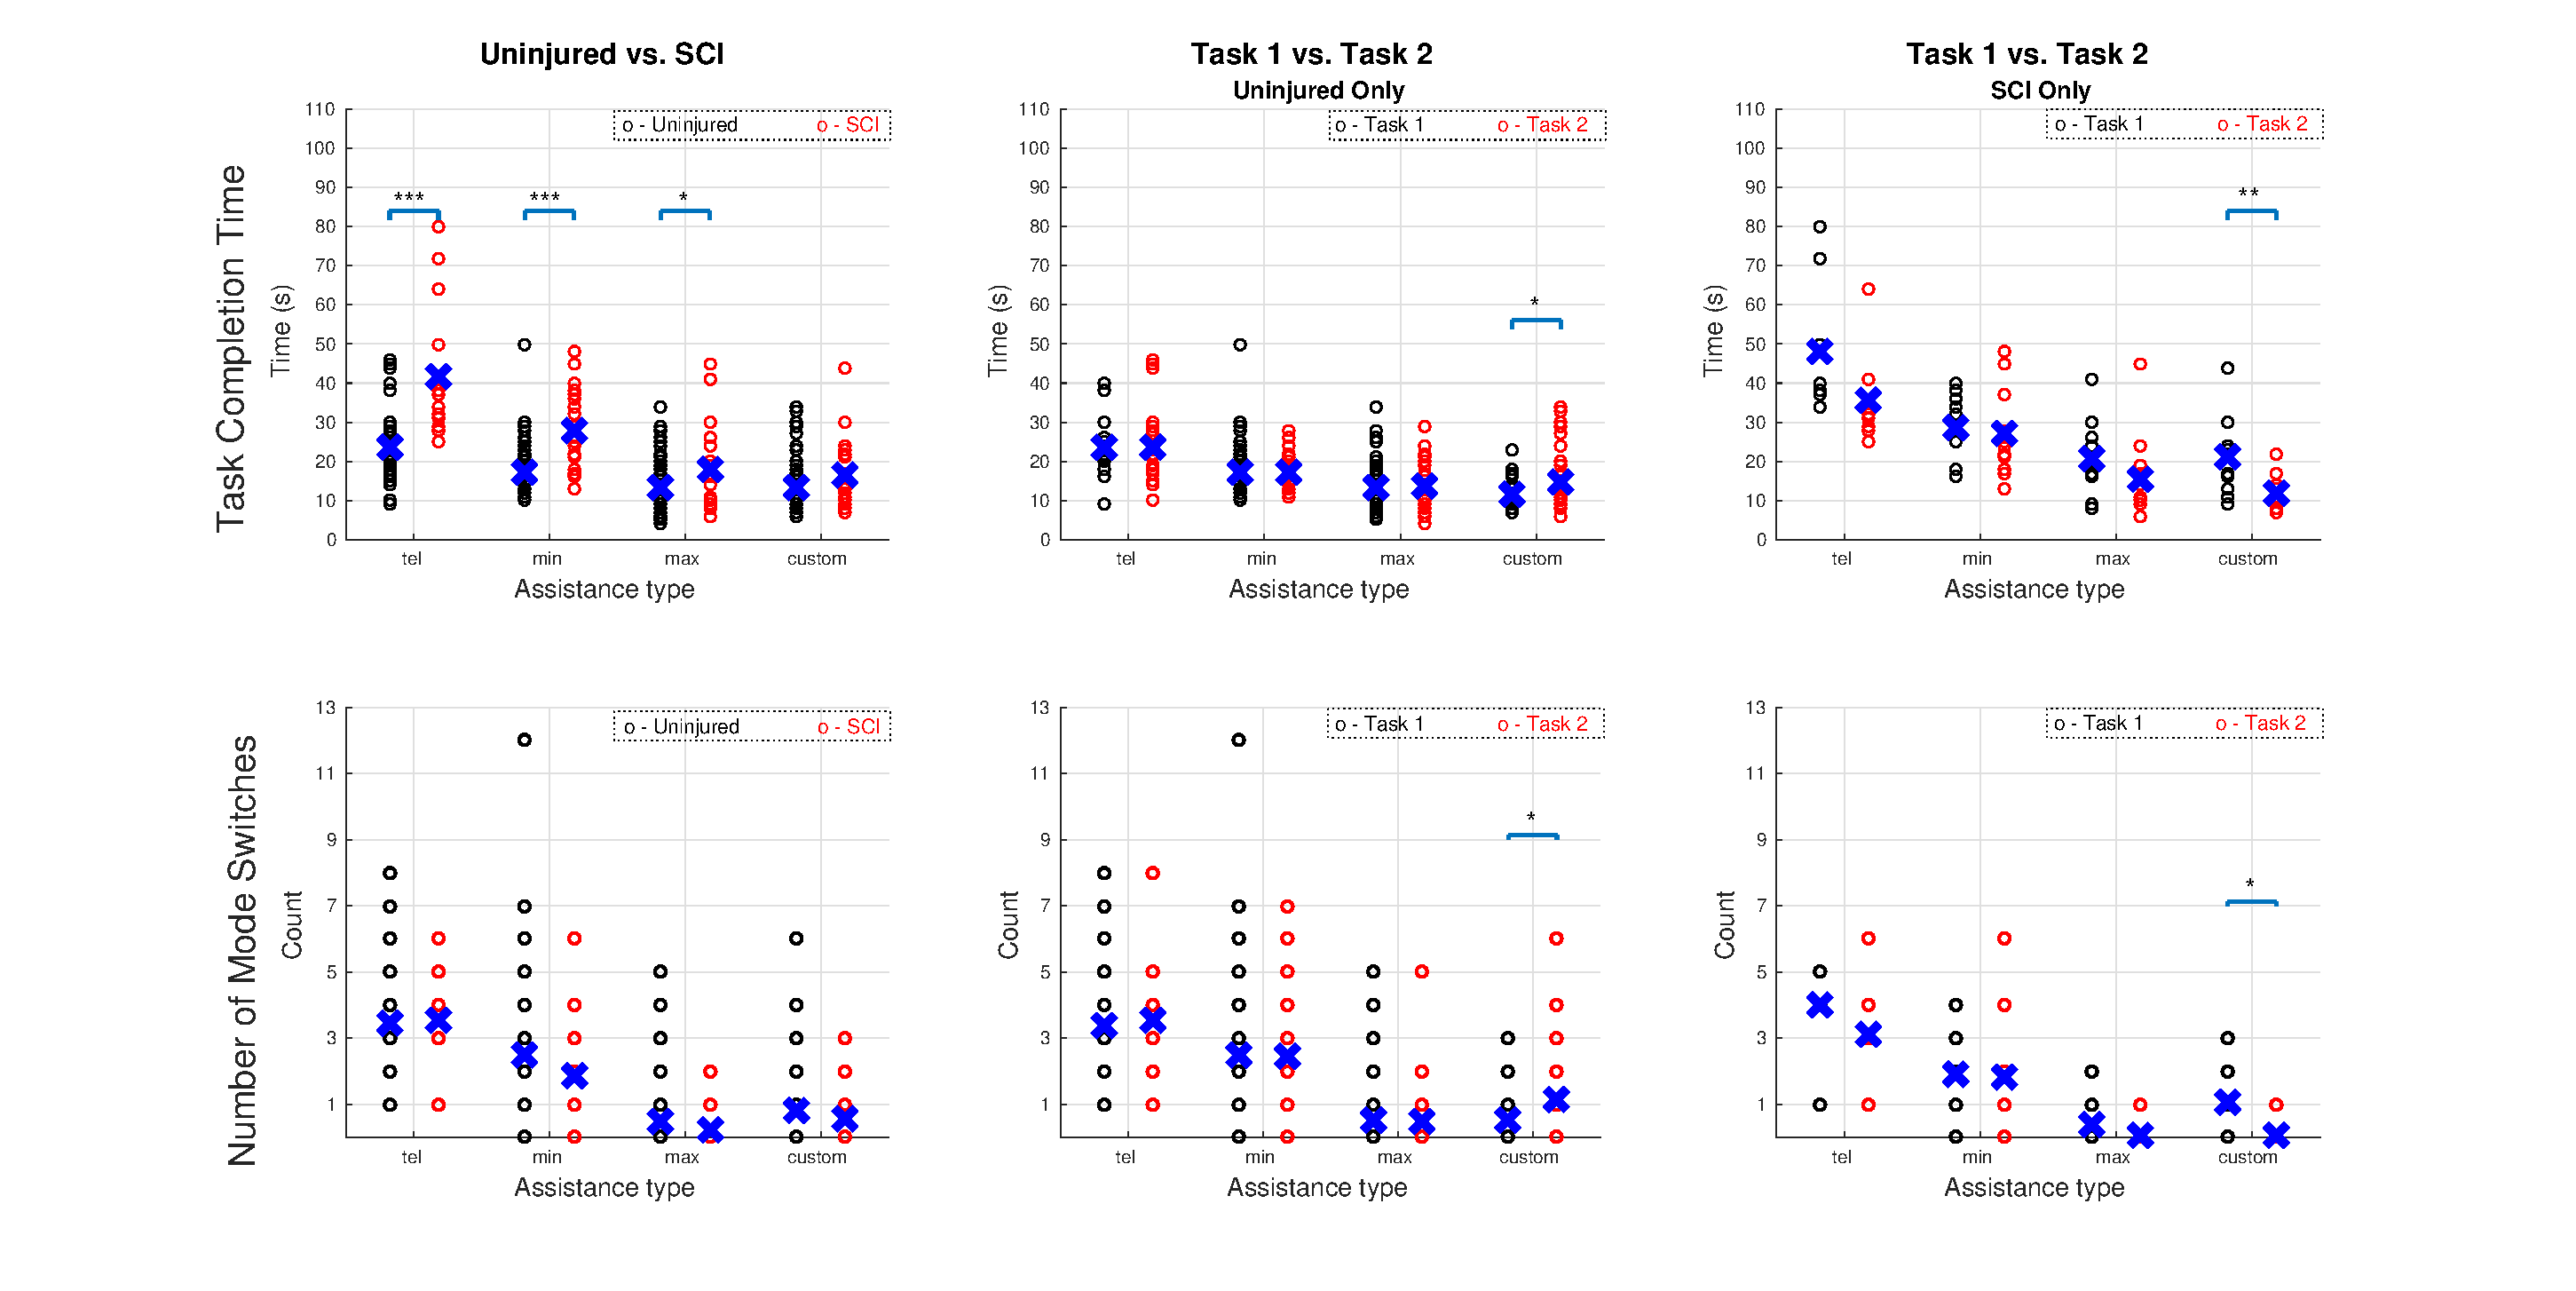
\includegraphics[width=1.18\hsize, center]{./finalfigures/Figure4.eps}
		\vspace{-1.1cm}
		\caption{Task completion time (top row) and number of mode switches (bottom row) for uninjured vs. SCI subjects (first column), Task 1 vs. Task 2 for uninjured subjects only (second column), Task 1 vs. Task 2 for SCI subjects only (third column).}
		\label{PlotOne}
	\end{figure*}
	\vspace{0.1cm}
	\noindent{\uline{\textit{Subjects:}}}  For this exploratory
	study 17 subjects were recruited---13 uninjured control subjects (mean
	age: $26 \pm 4$, 8 males and 5 females) and 4 spinal cord injury (SCI) subjects (mean age: $35 \pm 14$, all males, C3-C5 injury
	levels). Seven of the uninjured subjects (5 males, 2 females) and
	3 of the SCI subjects used the \textit{3D} interface paradigm, and the remaining
	subjects used the \textit{2D} paradigm.  All participants gave their
	informed, signed consent to participate in this experiment, which was
	approved by Northwestern University's Institutional Review Board.
	
	\vspace{0.1cm}
	\noindent{\uline{\textit{Protocol:}}} Each user performed all three
	tasks. The purpose of the practice task (R) was to get the user
	accustomed to the control interface and assistance system. Data was
	then collected on the remaining two tasks (RfG, RfS). The order of presentation
	for the RfG and RfS tasks was randomized and balanced across
	subjects, to avoid ordering effects.
	
	Before the RfG and RfS trials, the user was first asked to operate the system in full teleoperation mode (\textit{tel}) and also under three predefined assistance levels (\textit{min, mid} and \textit{max}). After this phase, the subject was given the option to customize the assistance level. Changes in assistance levels were communicated verbally to the system operator resulting in the parameter changes outlined in Table I. The user then tested the customized assistance level by executing the task. This customization procedure was repeated until the user was satisfied and lasted on average 10 and a maximum of 15 minutes, resulting in assistance level \textit{custom}. Data collection began only after this customization process was completed. Three trials were collected for \textit{min, max} and \textit{custom} assistance levels.\footnote{For one SCI participant one less trial was recorded for \textit{min} assistance level during the first task due to a clerical error.} A typical session lasted approximately 1-1.5 hours. 
	For the first (non-practice) task, the baseline from which customization began was the \textit{mid} level assistance, with level \textit{custom} being the result after customization. For the second task, customization began at this level \textit{custom} from the first task as the baseline, with the option to further customize resulting in level \textit{custom} for the second task.
	
	\noindent{\uline{\textit{Metrics:}}} A number of objective metrics evaluated this study. \textit{Task Completion time} was the amount of time spent accomplishing a task. \textit{Mode Switches} refers to the number of times the subject switched between the various modes of the control interface (Table \ref{tbl:modes}). Mode switches additionally is an indirect measure of the effort put forth by the user. At the
	end of the study, subjective data was gathered via a brief
	questionnaire. Users were given
	statements about the assistance system to rate on a 7-point Likert scale (1 is low, 7 is high), according to
	their agreement. The questions primarily concerned the utility value of the assistance system (\textit{U1}), the system's accuracy in goal perception (\textit{CA1}) and its understanding of what the user is trying to accomplish (\textit{CA2}), and the contribution from the user (\textit{CO1}) and the system (\textit{CO2}) in task accomplishment.
	
	\section{RESULTS} \label{RES}
	Here we report the results of our pilot study.\footnote{The video of the study can be found at \url{http://argallab.smpp.northwestern.edu/index.php/publications/}} An improvement in task performance with customization is demonstrated, and a number of other interesting observations are noted. Task performance metrics for different assistance levels (denoted by \textit{min}, \textit{max} and \textit{custom} in the plots) and teleoperation (\textit{tel)} are analyzed across different subject groups, tasks and control interfaces. Note that the \textit{custom} assistance level always lies in between (or is equal to) \textit{min} and \textit{max}. 
	Statistical significance is determined by Welch t-tests for Figures~\ref{PlotOne}-\ref{PlotTwo} and two sided Wilcoxon Rank-Sum Test for Figure~\ref{RCAP}, where (***) indicates $p<0.001$, (**) $p<0.01$ and (*) $p<0.05$.
	\subsection{Observations across Uninjured and SCI subjects}
	\noindent{\uline{\textit{Insight into Cost Function:}}}
	In this study, 17 subjects performed 34 rounds of customization in total. For 7 customization rounds the mean \textit{custom} task completion time was greater (by at least one standard error) than that of \textit{max}. Similarly, the number of mode switches for \textit{custom} was greater than that of \textit{max} for 14 customization rounds. This indicates that subjects are not always optimizing for standard performance metrics---because there does exist a parametrization (\textit{max}) which was known to the subjects and performs better with respect to these metrics.
	%\vspace*{-0.09cm}
	This  provides insight that the true cost function that the user is optimizing likely is more complex than a simple time-optimal or minimum-effort cost function. 
	
	\vspace{0.1cm}
	\noindent{\uline{\textit{Task Performance:}}} 
	In Figure \ref{PlotOne} (first column), the difference between uninjured and SCI subjects' task completion times drops steadily from \textit{tel} to \textit{custom} assistance levels. The t-tests revealed that while the difference between uninjured and SCI was statistically significant for \textit{tel} ($p$ = $5.1e$-$4$), \textit{min} ($p$ = $6.5e$-$5$) and \textit{max} ($p$ = $0.027$), this difference disappeared with the \textit{custom} ($p$ = $0.096$) assistance level. That is, with customized assistance, the performance of SCI subjects was \textit{statistically equivalent} to that of uninjured subjects. The variance in the data also \textit{decreases} with customized assistance, showing the performance to become more consistent. 
	
	Interestingly, for mode switches there was no statistical difference between uninjured and SCI subject data for any of the assistance levels. 
	This suggests that the number of mode switches is primarily determined by the nature of the task and control interface, and not the state of injury. However, SCI subjects do take more time than uninjured subjects to perform the same number of mode switches. 
	\vspace{-0.1cm}
	\subsection{Observations across Tasks}
	Figure \ref{PlotOne} (second and third columns) shows how task completion times and number of mode switches change between the first and second task for uninjured and SCI subjects. A statistically significant difference in performance only is observed for \textit{custom} assistance, for both groups. 
	Interestingly, SCI subjects show an \textit{improvement} in task completion times ($p$ = $7.8e$-$3$) and mode switches ($p$ = $8.9e$-$3$) between the first and second tasks, whereas uninjured subjects exhibit a performance \textit{decrease}. These changes in performance can be explained by the changes in assistance amount that result from the between-task customization (discussed further in Section~\ref{RCPC}).
	\begin{figure}[t]
		\centering
		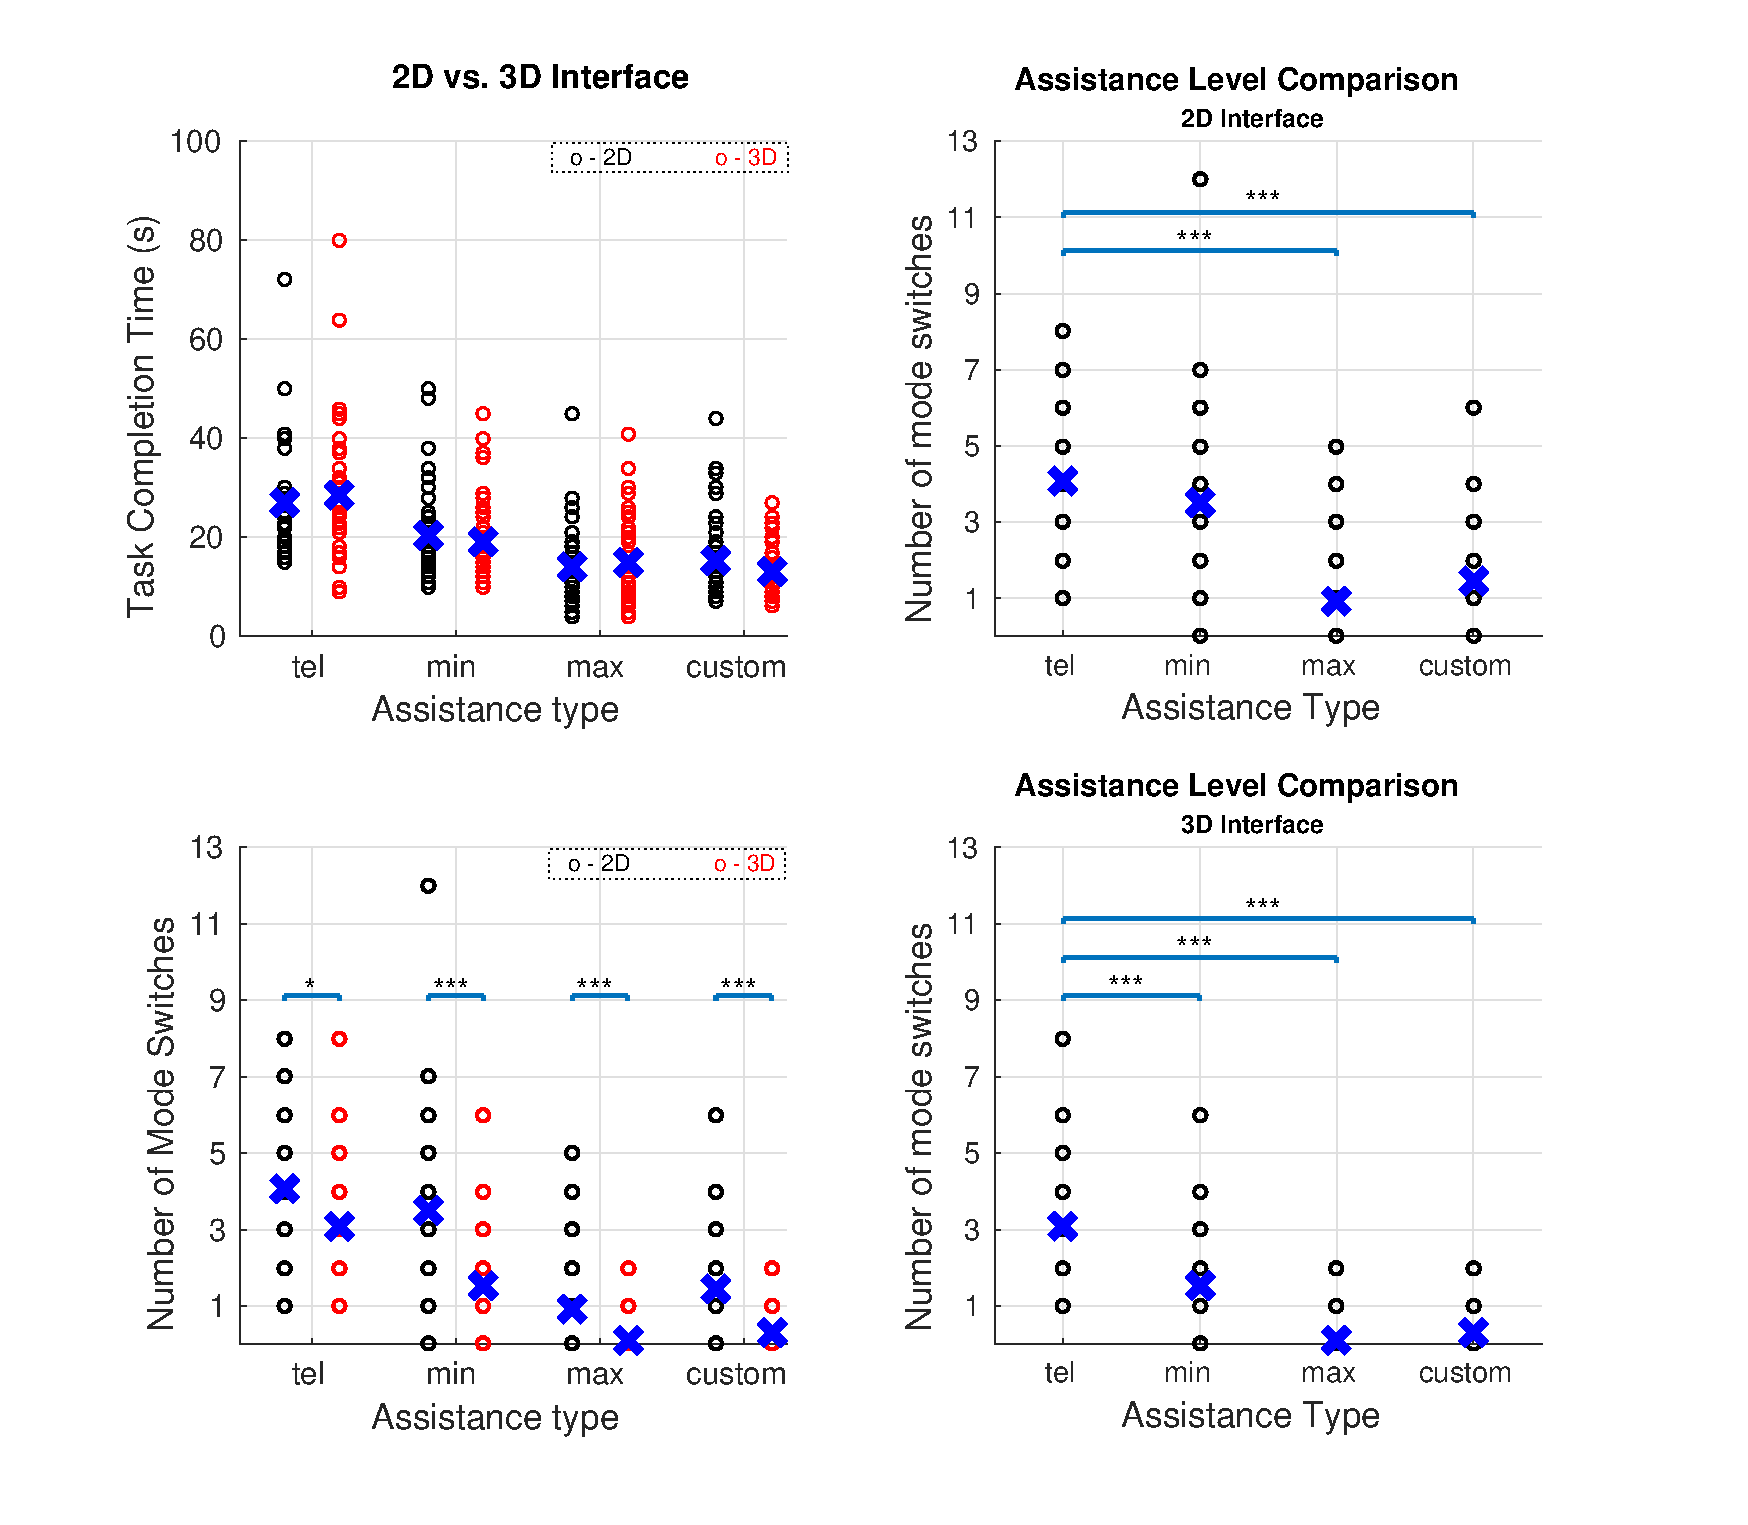
\includegraphics[width = 1.2\hsize, center]{./finalfigures/Figure5.eps}
		\vspace{-1.0cm}
		\caption{Left Column: Task completion time (top) and number of mode switches (bottom) for the 2D vs. 3D interfaces. Right Column: Within-interface assistance comparison for the 2D (top) and 3D (bottom) interfaces.}
		\label{PlotTwo}
	\end{figure}
	\subsection{Observations across Control Interfaces}
	Figure \ref{PlotTwo} (first column) shows the task completion times and mode switches for subjects using the \textit{2D} and \textit{3D} interfaces. Different operational modes do not seem to have an effect on task completion times, as both groups are statistically equivalent---\textit{despite} the fact that for mode switches the difference between the \textit{2D} and \textit{3D} interfaces is significant. The second column of Figure \ref{PlotTwo} shows a \textit{within-interface} performance comparison between \textit{tel} and the different assistance levels. For all levels assistance significantly helped in reducing the number of mode switches during task execution.
	
	The comparable task completion times may be explained by the fact that easier control compensates for time lost during mode switches. That is, due to the greater number of mode switches required for the \textit{2D} interface compared to the \textit{3D} interface, more time is taken performing mode switches. However, the number of dimensions simultaneously controlled is less for the \textit{2D} interface compared to the \textit{3D} interface, which makes the control easier.
	
	\subsection{Relative Change in Parameters during Customization} \label{RCPC}
	Figure~\ref{RCAP} shows the change in amount of assistance (parameter values) during customization for uninjured and SCI subjects. While SCI subjects on average increased the amount of assistance ($p$\;=\;$0.020$) during the second phase of customization, uninjured subjects chose to reduce the amount of assistance ($p$ = $0.006$). By contrast, there are no noticeable changes in the amount of assistance when using the \textit{2D} versus \textit{3D} interface. Injury thus seems to be the primary factor in how subjects choose to change the customized assistance level, and the mapping paradigm seems to have little effect. It furthermore is interesting that uninjured subjects chose to reduce assistance in spite of an associated decrease in task performance.
	\begin{figure}[t]
		\centering
		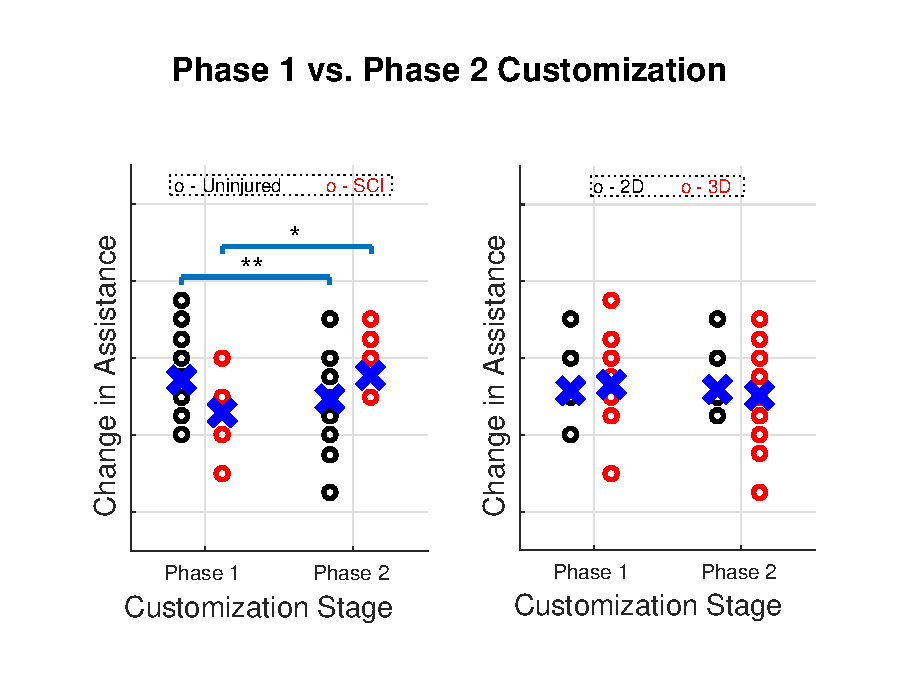
\includegraphics[scale=0.5]{./finalfigures/Figure6.eps}
		\vspace{-0.6cm}
		\caption{Relative change in assistance parameters during customization for Uninjured vs. SCI subjects (left) and 2D vs. 3D interfaces (right).}
		\label{RCAP}
	\end{figure}
	\subsection{User Survey}
	Users rated (Fig.~\ref{US}) the utility value of the assistance system fairly high (mean = $5.9\pm0.8$) indicating that in general having assistance was favored. The users also thought that the system was able to perceive goals accurately (mean = $5.1\pm1.8$) and the inability to estimate human intent was fairly low (mean = $3.1\pm1.1$). The users also felt that they played an important part in accomplishing the task (mean = $5.5\pm1.0$), almost comparable to the contribution from assistance (mean = $5.1\pm1.6$), maybe indicating that they were not prepared to relinquish control altogether.
	\begin{figure}[t]
		%	\centering
		\includegraphics[scale = 0.42, center]{./finalfigures/Figure7.eps}
		\vspace{-0.5cm}
		\caption{User responses on perceived utility, contribution and capability.}
		\label{US}
	\end{figure}
	\vspace{-0.08cm}
	\subsection{Discussion}
	From our pilot study we saw that compared to pre-defined assistance levels, customization improves task performance and helps to reduce performance differences between uninjured and SCI subjects. Post-experiment surveys also revealed that the users found the customized assistance paradigm to be useful. These results establish a need for customization of assistance levels. Therefore, our next step will be to explore multiple possibilities for building effective and intuitive customization mechanisms (e.g.~physical interfaces operated by the user) which will suit individual requirements and preferences, and to evaluate on a larger end-user population. The results also show that the true cost function that is being optimized is more complex than a simple time-optimal or minimum-effort cost function, indicating the need to investigate the exact specification of the true cost function that is being optimized by the human in a shared control system. A more comprehensive user survey will also be administered in which the formalized customization procedure will be evaluated thoroughly.
	%\addtolength{\textheight}{-0.1cm}  
%	\vspace{-0.2cm}
	\section{CONCLUSIONS}\label{CON}
	In this work, we formalized human robot interaction in shared autonomy within the framework of optimal control theory. Furthermore we introduced a system for user-driven customization as a constrained nonlinear optimization problem within this framework. Unlike standard optimization problems in which the form of the cost function is predetermined in this work no such assumptions were made. Instead, the end user was allowed to directly perform the optimization procedure. The aim is that this will lead to higher user satisfaction, which is crucial for the acceptance of novel technologies in the assistive domain. An interactive user-driven customization system was developed to ground the formalism and the results from the pilot study were presented. Results showed that all subjects were able to converge to a optimal assistance paradigm, and an improvement in task performance with customization also was demonstrated.
	\section*{ACKNOWLEDGMENTS}\label{ACK}
	Many thanks to Jessica Presperin Pedersen, OTR/L,
	ATP/SMS, for recruiting the SCI subjects, and to Samuel
	Schlesinger for assistance during the subject studies. The content is solely
	the responsibility of the authors and does not necessarily
	represent the official views of the NIH.
	
\balance	
\bibliographystyle{ieeetr}
\bibliography{GopinathJainArgall_RAL}






\end{document}
